%%%%%%%%%%%%%%%%%%%%%%%%%%%%%%%%%%%%%%%%%%%%%%%%%%%%%%%%%%%%%%%%%%%%%%%%%%%%%%%
\documentclass[hyperref={pdfpagelabels=false},compress,table]{beamer} % 在Mac下无法编译
% \documentclass[compress,table]{beamer} % 在Mac下使用
% package for font
\usepackage{fontspec}
\defaultfontfeatures{Mapping=tex-text}  %%如果没有它,会有一些 tex 特殊字符无法正常使用,比如连字符。
\usepackage{xunicode,xltxtra}
\usepackage[BoldFont,SlantFont,CJKnumber,CJKchecksingle]{xeCJK}  % \CJKnumber{12345}: 一万二千三百四十五
\usepackage{CJKfntef}  %%实现对汉字加点、下划线等。
\usepackage{pifont}  % \ding{}
% package for math
\usepackage{amsfonts}

% package for graphics
\usepackage[americaninductors,europeanresistors]{circuitikz}
\usepackage{tikz}
\usetikzlibrary{plotmarks}  % placements=positioning
\usepackage{graphicx}  % \includegraphics[]{}
\usepackage{subfigure}  %%图形或表格并排排列
% package for table
\usepackage{colortbl,dcolumn}  %% 彩色表格
\usepackage{multirow}
\usepackage{multicol}
\usepackage{booktabs}
% package for code
\usepackage{fancyvrb}
\usepackage{listings}

% \usepackage{animate}
% \usepackage{movie15}

%%%%%
% setting for beamer
\usetheme{default} % Madrid(常用), Copenhagen, AnnArbor, boxes(白色), Frankfurt,Berkeley
\useoutertheme[subsection=true]{miniframes} % 使用Berkeley时注释本行
\usecolortheme{sidebartab}
\usefonttheme{serif}  %%英文使用衬线字体
% \setbeamertemplate{background canvas}[vertical
% shading][bottom=white,top=structure.fg!7] %%背景色,上25%的蓝,过渡到下白。
\setbeamertemplate{theorems}[numbered]
\setbeamertemplate{navigation symbols}{}  %% 去掉页面下方默认的导航条
\setbeamercovered{transparent}  %设置 beamer 覆盖效果

% 设置标题title背景色
% \setbeamercolor{title}{fg=black, bg=lightgray!60!white}
\setbeamercolor{title}{fg=white, bg=black!70!white}

% 设置每页小LOGO
\pgfdeclareimage[width=1cm]{ouc}{figures/static/ouc.pdf}
\logo{\pgfuseimage{ouc}{\vspace{-20pt}}}

% setting for font
%%\setCJKmainfont{Adobe Kaiti Std}
\setCJKmainfont{SimSun} 
%% \setCJKmainfont{FangSong_GB2312} 
%% \setmainfont{Apple Garamond}  %%苹果字体没有SmallCaps
\setCJKmainfont{SimSun} 
%FUNNY%\setCJKmainfont{DFPShaoNvW5-GB}  %%华康少女文字W5(P)
%FUNNY%\setCJKmainfont{FZJingLeiS-R-GB}  %%方正静蕾体
%FUNNY%\setmainfont{Purisa}
%\setsansfont[Mapping=tex-text]{Adobe Song Std}
     %如果装了Adobe Acrobat,可在font.conf中配置Adobe字体的路径以使用其中文字体。
     %也可直接使用系统中的中文字体如SimSun、SimHei、微软雅黑等。
     %原来beamer用的字体是sans family;注意Mapping的大小写,不能写错。
     %设置字体时也可以直接用字体名,以下三种方式等同:
     %\setromanfont[BoldFont={黑体}]{宋体}
     %\setromanfont[BoldFont={SimHei}]{SimSun}
     %\setromanfont[BoldFont={"[simhei.ttf]"}]{"[simsun.ttc]"}
% setting for graphics
\graphicspath{{figures/}}  %%图片路径
\renewcommand\figurename{图}

% setting for pdf
\hypersetup{% pdfpagemode=FullScreen,%
            pdfauthor={Xiaodong Wang},%
            pdftitle={Title},%
            CJKbookmarks=true,%
            bookmarksnumbered=true,%
            bookmarksopen=false,%
            plainpages=false,%
            colorlinks=true,%
            citecolor=green,%
            filecolor=magenta,%
            linkcolor=blue,%red(default)
            urlcolor=cyan}

% setting for fontspec
\XeTeXlinebreaklocale "zh"  %%表示用中文的断行
\XeTeXlinebreakskip = 0pt plus 1pt minus 0.1pt  %%多一点调整的空间
%%%%%

% font setting by xeCJK
\setCJKfamilyfont{NSimSun}{NSimSun}
\newcommand{\song}{\CJKfamily{NSimSun}}
%%%\setCJKfamilyfont{AdobeSongStd}{Adobe Song Std}
%%%\newcommand{\AdobeSong}{\CJKfamily{AdobeSongStd}}
\setCJKfamilyfont{FangSong}{FangSong_GB2312}
\newcommand{\fang}{\CJKfamily{FangSong}}
%%%\setCJKfamilyfont{AdobeFangsongStd}{Adobe Fangsong Std}
%%%\newcommand{\AdobeFang}{\CJKfamily{AdobeFangsongStd}}
\setCJKfamilyfont{SimHei}{SimHei}
\newcommand{\hei}{\CJKfamily{SimHei}}
%%%\setCJKfamilyfont{AdobeHeitiStd}{Adobe Heiti Std}
%%%\newcommand{\AdobeHei}{\CJKfamily{AdobeHeitiStd}}
\setCJKfamilyfont{KaiTi}{KaiTi}
\newcommand{\kai}{\CJKfamily{KaiTi}}
%%%\setCJKfamilyfont{AdobeKaitiStd}{Adobe Kaiti Std}
\newcommand{\AdobeKai}{\CJKfamily{AdobeKaitiStd}}
\setCJKfamilyfont{LiSu}{LiSu}
\newcommand{\li}{\CJKfamily{LiSu}}
\setCJKfamilyfont{YouYuan}{YouYuan}
\newcommand{\you}{\CJKfamily{YouYuan}}
\setCJKfamilyfont{FZJingLei}{FZJingLeiS-R-GB}
\newcommand{\jinglei}{\CJKfamily{FZJingLei}}
\setCJKfamilyfont{MSYH}{Microsoft YaHei}
\newcommand{\msyh}{\CJKfamily{MSYH}}

% 自定义颜色
\def\Red{\color{red}}
\def\Green{\color{green}}
\def\Blue{\color{blue}}
\def\Mage{\color{magenta}}
\def\Cyan{\color{cyan}}
\def\Brown{\color{brown}}
\def\White{\color{white}}
\def\Black{\color{black}}

\lstnewenvironment{xmlCode}[1][]{% for Java
  \lstset{
    basicstyle=\tiny\ttfamily,%
    columns=flexible,%
    framexleftmargin=.7mm, %
    % frame=shadowbox,%
    % rulesepcolor=\color{cyan},%
     frame=single,%
    backgroundcolor=\color{white},%
    xleftmargin=4\fboxsep,%
    xrightmargin=4\fboxsep,%
    numbers=left,numberstyle=\tiny,%
    numberblanklines=false,numbersep=7pt,%
    language=xml, %
    }\lstset{#1}}{}

\lstnewenvironment{javaCode}[1][]{% for Java
  \lstset{
    basicstyle=\tiny\ttfamily,%
    columns=flexible,%
    framexleftmargin=.7mm, %
    frame=shadowbox,%
    rulesepcolor=\color{cyan},%
    % frame=single,%
    backgroundcolor=\color{white},%
    xleftmargin=4\fboxsep,%
    xrightmargin=4\fboxsep,%
    numbers=left,numberstyle=\tiny,%
    numberblanklines=false,numbersep=7pt,%
    language=Java, %
    }\lstset{#1}}{}

\lstnewenvironment{shCode}[1][]{% for Java
  \lstset{
    basicstyle=\scriptsize\ttfamily,%
    columns=flexible,%
    framexleftmargin=.7mm, %
    frame=shadowbox,%
    rulesepcolor=\color{brown},%
    % frame=single,%
    backgroundcolor=\color{white},%
    xleftmargin=4\fboxsep,%
    xrightmargin=4\fboxsep,%
    numbers=left,numberstyle=\tiny,%
    numberblanklines=false,numbersep=7pt,%
    language=sh, %
    }\lstset{#1}}{}

\newcommand\ask[1]{\vskip 4bp \tikz \node[rectangle,rounded corners,minimum size=6mm,
  fill=white,]{\Cyan \includegraphics[height=1.5cm]{question} \Large \msyh #1};}

\newcommand\wxd[1]{\vskip 4bp \tikz \node[rectangle,minimum size=6mm,
  fill=blue!60!white,]{\White \ding{118} \msyh #1};}

\newcommand\xyy[1]{\vskip 2bp \tikz \node[rectangle,minimum size=3mm,
  fill=black!80!white,]{\White \msyh\scriptsize #1};}

\newcommand\homework[1]{\vskip 2bp \tikz \node[rectangle,minimum size=3mm,
  fill=red!80!white,]{\White \ding{45} \msyh\scriptsize 课后小作业 } ; {\kai\small #1}} 

\newcommand\cxf[1]{\vskip 4bp \tikz \node[rectangle,rounded corners,minimum size=6mm,
  fill=purple!60!white,]{\White \ding{42} \msyh #1};}

\newcommand\tta[1]{\vskip 4bp \tikz \node[rectangle,minimum size=6mm,
  fill=blue!60!white,]{\White \ding{118} \msyh #1};}

\newcommand\ttb[1]{\vskip 4bp \tikz \node[rectangle,rounded corners,minimum size=6mm,
  fill=purple!60!white,]{\White \ding{42} \msyh #1};}

\newcommand\ttc[1]{\vskip 2bp \tikz \node[rectangle,minimum size=3mm,
  fill=black!80!white,]{\White \msyh\scriptsize #1};}

\newcommand\notice[1]{\vskip 4bp \tikz \node[rectangle,rounded corners,minimum size=6mm,
  fill=red!80!white,]{\White \scriptsize \ding{42} \msyh #1};}

\newcommand\samp[1]{\vskip 2bp \tikz \node[rectangle,minimum size=3mm,
  fill=white!100!white,]{\Mage\msyh \small CODE \ding{231} \Black #1};\vskip -8bp}

\newcommand\codeset[1]{\vskip 2bp \tikz \node[rectangle,minimum size=3mm,
  fill=white!100!white,]{\Mage\msyh \small 课程配套代码 \ding{231} \Black #1};\vskip -8bp}

\newcommand\pptlink[2]{\vskip 4bp \tikz \node[rectangle,rounded corners,minimum size=6mm,
  fill=blue!70!white,]{\href{run:#1}{\White \scriptsize \msyh 动画演示 #2}};}



\setbeamerfont{frametitle}{series=\msyh} % 修改Beamer标题字体

\makeatletter
\newcommand{\Extend}[5]{\ext@arrow 0099{\arrowfill@#1#2#3}{#4}{#5}}
\makeatother


%%%%%%%%%%%%%%%%%%%%%%%%%%%%%%%%%%%%%%%%%%%%%%%%%%%%%%%%%%%%%%%%%%%%%%%%%%%%%%%
% \titlepage
\title[Wang Xiaodong]{\hei {\huge Java 应用与开发}\\  
  Java技术概述及开发环境}
\author[王晓东]{王晓东\\
  \href{mailto:wangxiaodong@ouc.edu.cn}{\footnotesize wangxiaodong@ouc.edu.cn}}
\institute[中国海洋大学]{\small 中国海洋大学}
\date{\today}
\titlegraphic{\vspace{-6em}
\includegraphics[height=6cm]{static/ouc.pdf}\vspace{-6em}}
%%%%%%%%%%%%%%%%%%%%%%%%%%%%%%%%%%%%%%%%%%%%%%%%%%%%%%%%%%%%%%%%%%%%%%%%%%%%%%%
\begin{document}
%% Delete this, if you do not want the table of contents to pop up at
%% the beginning of each subsection:
\AtBeginSection[]{                              % 在每个Section前都会加入的Frame
  \frame<handout:0>{
    \frametitle{\textbf{\hei 接下来…}}
    \tableofcontents[currentsection]
  }
}  %

\AtBeginSubsection[]                            % 在每个子段落之前
{
  \frame<handout:0>                             % handout:0 表示只在手稿中出现
  {
    \frametitle{\textit{\hei 接下来…}}\small
    \tableofcontents[current,currentsubsection] % 显示在目录中加亮的当前章节
  }
}
 \frame{\titlepage}

%%%%%%%%%%%%%%%%%%%%%%%%%%%%%%%%%%%%%%%%%%%%%%%%
\begin{frame}
\frametitle{参考书目}
\begin{enumerate}
\item 陈国君等编著, Java程序设计基础(第5版), 清华大学出版社
\item Bruce Eckel, Thinking in Java (3rd)
\end{enumerate}  
\end{frame}

\begin{frame}
\frametitle{学习目标}
\begin{enumerate}
\item 了解Java的发展历程
\item 理解Java平台的相关概念和机制
\item 掌握基本Java开发环境配置
\end{enumerate}  
\end{frame}

\section*{大纲}
\frame{\frametitle{大纲} \tableofcontents }

\section{Java技术概述}
\begin{frame}[fragile] % [fragile]参数使得能够插入代码
  \frametitle{那些伟大的LOGO}
  \begin{figure}
    \centering
    \fbox{\includegraphics[width=0.4\textwidth]{sun_logo.jpg}}
  \end{figure}
  \begin{figure}
    \centering
    \fbox{\includegraphics[width=0.3\textwidth]{java-logo.jpg}}
  \end{figure}
  \begin{figure}
    \centering
    \fbox{\includegraphics[width=0.5\textwidth]{oracle_logo.jpg}}
  \end{figure}
\end{frame}

\begin{frame}[fragile] % [fragile]参数使得能够插入代码
\frametitle{Sun公司大事记}
\begin{description}\msyh\small
\item[\fbox{1982}] Sun公司成立(安迪$\cdot$贝托谢姆和麦克尼利)。
\item[\fbox{1986}] Sun公司上市。
\item[\fbox{1985}] Sun公司推出著名的Java语言。
\item[\fbox{2001}] 9.11事件前,Sun市值超过1000亿美元;此后,由于互联网泡沫的破碎,其市值
  在一个月内跌幅超过90\%。
\item[\fbox{2004}] Sun公司和微软在旷日持久的Java官司中和解,后者支付前者高达10亿美元的
  补偿费。
\item[\fbox{2006}] 共同创始人麦克尼利辞去CEO一职,舒瓦茨担任CEO后尝试将Sun从设备公司向软
  件服务型公司转型,但不成功。
\item[\fbox{2010}] Sun公司被甲骨文公司收购。
\end{description}
\end{frame}

\begin{frame}[fragile] % [fragile]参数使得能够插入代码
\frametitle{Java发展简史}
\begin{figure}
\centering
\includegraphics[width=0.80\textwidth]{java-father-gosling.jpg}
\caption{Java之父 詹姆斯·高斯林(James Gosling)}
\end{figure}
\end{frame}

\begin{frame}[fragile] % [fragile]参数使得能够插入代码
\frametitle{Java发展简史}
\begin{figure}
\centering
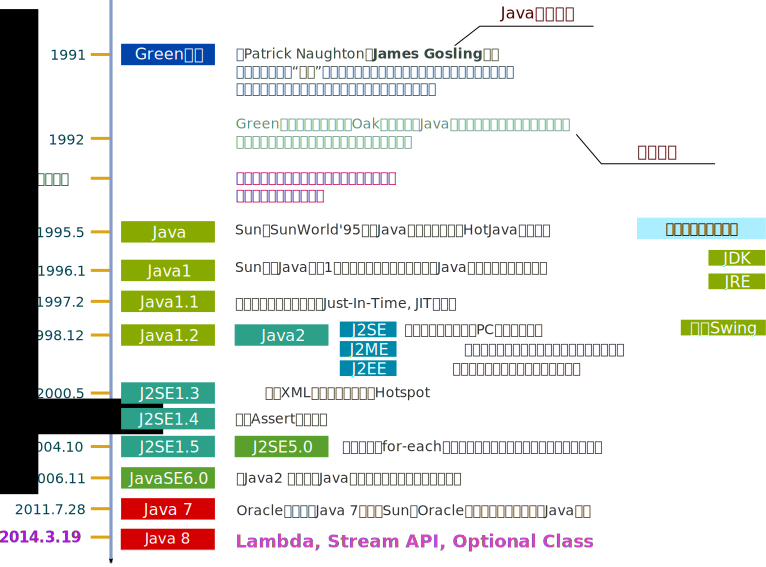
\includegraphics[width=0.95\textwidth]{fig01-01.pdf}
\end{figure}
\end{frame}

\begin{frame}[fragile]
\frametitle{Java技术的特点}
\begin{description}[<+-| alert@+>]\kai
\item[面向对象] \only<1>{Java是一种以对象为中心,以消息为驱动的面向对象
    的编程语言。}
\item[平台无关性] \only<2>{分为源代码级(需重新编译源代码,如C/C++)和
    目标代码级(Java)平台无关。}
\item[分布式] 
\item[可靠性] \only<4>{不支持直接操作指针,避免了对内存的非法访问;自动
    单元回收功能防止内存丢失等动态内存分配导致的问题;解释器运行时实施
    检查,可发现数组和字符串访问的越界;提供了异常处理机制。安全性。}
\item[多线程] \only<5>{C++没有内置的多线程机制,需调用操作系统的多线程
    功能来进行多线程序设计;Java提供了多线程支持。}
\item[网络编程]
\item[编译和解释并存] \only<7>{由编译器将Java源程序编译成字节码文件,再
    由运行系统解释执行字节码文件(解释器将字节码再翻译成二进制码运行)。}
\end{description}
\end{frame}

\section{Java平台核心机制}
\begin{frame}[fragile] % [fragile]参数使得能够插入代码
\frametitle{Java平台}
\begin{figure}
\centering
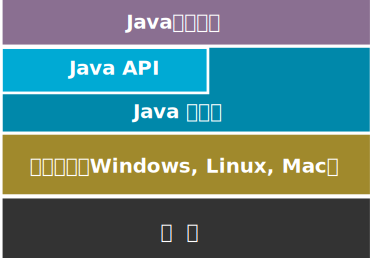
\includegraphics[width=0.5\textwidth]{fig02.pdf}
\end{figure}
\wxd{核心概念}
\begin{itemize}
\item Java虚拟机
\item 垃圾回收机制
\item Java运行时环境(Java Runtime Environment, JRE)
\end{itemize}
\end{frame}

\begin{frame}[fragile] % [fragile]参数使得能够插入代码
\frametitle{Java程序的运行过程}
\begin{figure}
\centering
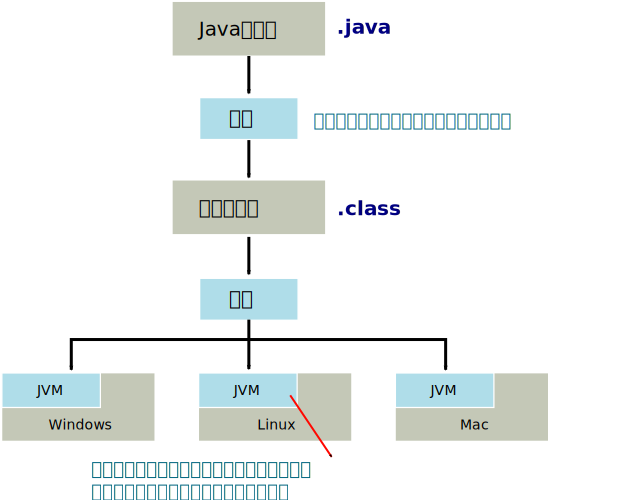
\includegraphics[width=0.65\textwidth]{fig03.pdf}
\end{figure}
\xyy{JIT, Just-In-Time} {\scriptsize 传统解释器的解释执行是转换一条,运行完后就将其扔掉;
  JIT会自动检测指令的运行情况,并将使用频率高(如循环运行)的指令解释后保存下来,下次调用
  时就无需再解释(相当于局部的编译执行),显著提高了Java的运行效率。}
\end{frame}

\section{Java开发环境}
\begin{frame}[fragile] % [fragile]参数使得能够插入代码
\frametitle{获取和安装Java开发工具集}
\wxd{Download}\\
http://www.oracle.com/technetwork/java/javase/downloads/index.html
\wxd{Install}\\
\begin{shCode}
D:\Program Files\Java
\end{shCode}
\begin{shCode}
/opt/jdk1.8.0_172
\end{shCode}
\wxd{Environment Variable}\\
\begin{description}
\item[\fbox{变量名}] Path
\item[\fbox{变量值}] D:\textbackslash Program Files\textbackslash Java\textbackslash
  jdk1.8.0\_172\textbackslash bin
\end{description}
\end{frame}

\begin{frame}[fragile] % [fragile]参数使得能够插入代码
\frametitle{获取和安装Java开发工具集}
\wxd{JDK Directories}\\
\begin{shCode}
  bin  COPYRIGHT  db  include  javafx-src.zip
  jre  lib  LICENSE  man  README.html  release  src.zip
  THIRDPARTYLICENSEREADME-JAVAFX.txt  THIRDPARTYLICENSEREADME.txt  
\end{shCode}
\begin{description}\scriptsize
\item[\fbox{bin}] Java开发工具,包括编译器、虚拟机、调试器、反编译器等;
\item[\fbox{jre}] Java运行时,包括Java虚拟机、类库和其他资源文件;
\item[\fbox{lib}] 类库和所需支持性文件;
\item[\fbox{include}] 用于调试本地方法(底层平台)的C++头文件;
\item[\fbox{src.zip}] 类库的源代码;
\item[\fbox{db}] Java DB数据库,JDK6.0新增项目,一种纯Java的关系型数据库;
\end{description}
\end{frame}

\begin{frame}[fragile] % [fragile]参数使得能够插入代码
\frametitle{Java开发工具}
\begin{itemize}
\item Notepad
\item Vim、Emacs
\begin{figure}
\centering
\includegraphics[width=0.4\textwidth]{java-emacs.png}
\end{figure}
\item {\Red Eclipse}
\begin{figure}
\centering
\includegraphics[width=0.4\textwidth]{java-Eclipse.png}
\end{figure}
\end{itemize}
\end{frame}

\section{Java基本开发流程}
\begin{frame}[fragile] % [fragile]参数使得能够插入代码
\frametitle{Java基本开发流程}
\begin{enumerate}[<+-| structure@+>]
\item 创建源文件HelloWorld.java,文件命名必须与类名相同。
\begin{javaCode}
public class HelloWorld {
    public static void main(String[] args) {
	System.out.println("Hi, Java!");
    }
}   
\end{javaCode}
\item 将源文件编译为字节码文件
\begin{shCode}
> javac HelloWorld.java && ls 
HelloWorld.class  HelloWorld.java
\end{shCode}
\item 运行程序
\begin{shCode}
> java HelloWorld 
Hi, Java!
\end{shCode}
\end{enumerate}
\end{frame}

\begin{frame}[fragile] % [fragile]参数使得能够插入代码
\frametitle{Java应用程序结构需掌握的几条规则}

\begin{enumerate}[<+-| alert@+>]
\item Java语言拼写是大小写敏感的(Case-Sensitive);
\item 一个源文件中可以定义多个Java类,但其中最多只能有一个类被定义为Public类;
\item 如果源文件中包含了public类,则源文件必须和该public类同名;
\item 一个源文件包含多个Java类时,编译后会生成多个字节码文件,即每个类都会生成一个单独的
  “.class”文件,且文件名与类名相同。
\end{enumerate}
\end{frame}

\begin{frame}
 \frametitle{本节习题}
 \begin{enumerate}
 \item 安装配置Eclipse Java开发环境
 \item 使用一个文本编辑器(记事本等)编写一个简单的Java程序,并从命令行编译执行该程序
 \end{enumerate}
\end{frame}
%%%%%%%%%%%%%%%%%%%%%%%%%%%%%%%%%%%%%%%%%%%%%%%%%%%%%%%%%%%%%%%%%%%%%%%%%%%%%%%
% TKS Page %%%%%%%%%%%%%%%%%%%%%%%%%%%%%%%%%%%%%%%%%%%%
\begin{frame}
\centering
{\Huge \textcolor{blue}{THE END}} \\
\vspace{5mm}
{\Large wangxiaodong@ouc.edu.cn} \\
\end{frame}
%%%%%%%%%%%%%%%%%%%%%%%%%%%%%%%%%%%%%%%%%%%%%%%%%%%%%%%
%%%%%%%%%%%%%%%%%%%%%%%%%%%%%%%%%%%%%%%%%%%%%%%%%%%%%%%%%%%%%%%%%%%%%%%%%%%%%%%
\end{document}
